\documentclass{ctexart}
\usepackage{hyperref}
\hypersetup{
	colorlinks=true,
	linkcolor=black,
	filecolor=blue,      
	urlcolor=blue,
	citecolor=cyan,
}
\usepackage{amsmath}
\usepackage{graphicx}
\usepackage{float}
\usepackage{listings}
\usepackage{xcolor}

\title{C++11实践指南学习笔记}
\author{fangcun}
\begin{document}
\maketitle
\newpage
\setcounter{tocdepth}{3}
\tableofcontents

\newpage
\section{序}

对于许多富有经验的程序员来说,他们想了解的并非是C++11的语法,而是实践中这样做的动机。本文就来自于一位C++专家的C++11实践经验总结,如果读者的英文不错,可以直接阅读英文原文:\href{https://stuartwheaton.com/blog/2020-06-14-c++11-guide/}{原文链接}。

\newpage
\section{重大改进}

C++11标准对C++有不少影响深远的改进,其中最重要的便是:移动语义(Move Semantics)、智能指针(Smart Pointers)、哈希表和集合(Hash Maps and Sets)。

\subsection{移动语义}

移动语义(Move Semantics)应该是C++11标准带来的最大改进。通过移动语义,我们可以实现更为细致的内存管理。比如,从一个之后不再使用的对象复制数据时,我们可以通过移动语义手动回收利用这个对象可以被我们直接利用的内存数据,避免大规模的内存复制操作。这对于移动操作的时间复杂度是常数时间的情况(vector,map,unordered\_map,string等标准库对象都是这样),我们的性能收益是巨大的。那么,问题是我们如何知道一个对象在之后不再使用?这就需要了解右值(rvalue)的概念,它表示一个临时的,在之后不能被访问的值。对于下面的代码,user是一个左值(lvalue),字符串字面量"Skywalker"是一个右值(rvalue)。我们可以在这行代码运行之后访问user变量,但却不能访问到原始的字符串字面量"Skywalker"(读者思考下为什么?)。

\begin{lstlisting}[language={[ANSI]C},keywordstyle=\color{blue!70},commentstyle=\color{red!50!green!50!blue!50},frame=shadowbox, rulesepcolor=\color{red!20!green!20!blue!20},basicstyle=\small,numbers=left, numberstyle=\tiny,breaklines=true]
string user("Skywalker");
\end{lstlisting}

下图通过一个生活中的场景来说明移动语义(Move Semantics)。图1中,蓝色小人通过复制构造复制(重新生成或初始化,生成和初始化需要耗费大量时间)了红色小人房子里的家具,图2中,蓝色小人通过移动构造继承了红色小人房子里的家具。显然,对于蓝色小人来说,继承红色小人的家具比自己购买新的一模一样的家具的代价要小(不用花钱:-) ),换成代码来说,就是继承比复制更高效。

\begin{figure}[H]
	\title{图1:复制构造会重新生成每个家具}
	\centering
	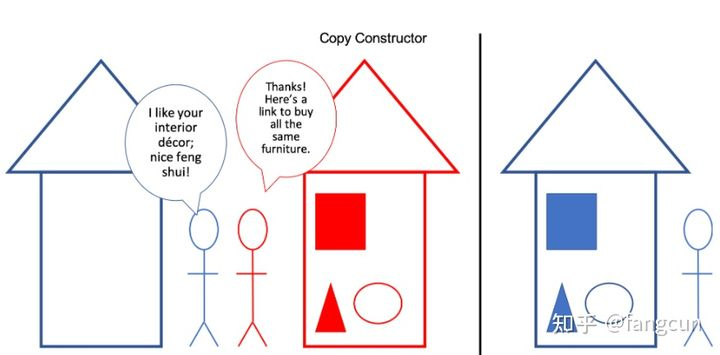
\includegraphics[scale=0.5]{img/1-1.jpg}
\end{figure}

\begin{figure}[H]
	\title{图2:移动构造直接转移每个家具,不存在重新生成和初始化的时间成本}
	\centering
	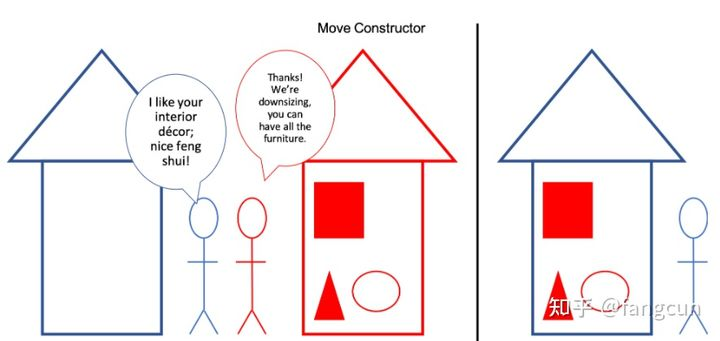
\includegraphics[scale=0.5]{img/1-2.jpg}
\end{figure}

下面给出了复制构造和移动构造的一个示例代码,当要复制的对象是一个右值(rvalue),会调用移动构造函数,其它情况调用复制构造函数。可以看出,一个典型的复制构造函数和典型的移动构造函数之间的不同:移动构造函数的参数没有使用const关键字,参数的变量名前有两个\&符号,用来表示右值引用。因为rhs是右值引用,我们可以认为在之后它不会再被使用,所以移动构造函数直接复制了对象数据的内存指针,没有进行内存分配和数据的深copy。除了移动构造函数,我们还可以在赋值运算上使用移动语义。

\begin{lstlisting}[language={[ANSI]C},keywordstyle=\color{blue!70},commentstyle=\color{red!50!green!50!blue!50},frame=shadowbox, rulesepcolor=\color{red!20!green!20!blue!20},basicstyle=\small,numbers=left, numberstyle=\tiny,breaklines=true]
// Copy constructor  
string(const string& rhs) {  
	allocateSpace(myDataPtr);  
	deepcopy(rhs.myDataPtr, myDataPtr);  
}  
// Move constructor  
string(string&& rhs) {  
	myDataPtr = rhs.myDataPtr;  
	rhs.myDataPtr = nullptr;  
}
\end{lstlisting}

对于一个可引用的变量(lvalue),如果我们确定之后不会再使用它,可以使用std::move手动将其变为右值参数。有时候,我们还会让对象只能进行移动操作不能进行复制操作。对于被移动的对象,如果没有重新初始化,我们不应该使用它。下面的代码演示了这一个过程,标准库中的unique\_ptr类生成的对象就是一个只能移动,不能复制的对象。

\begin{lstlisting}[language={[ANSI]C},keywordstyle=\color{blue!70},commentstyle=\color{red!50!green!50!blue!50},frame=shadowbox, rulesepcolor=\color{red!20!green!20!blue!20},basicstyle=\small,numbers=left, numberstyle=\tiny,breaklines=true]
MoveOnlyObject a;
...  
MoveOnlyObject b(a); // ERROR – copy constructor doesn't exist
MoveOnlyObject c(std::move(a)); // OK – ownership transferred to c. a is DEAD now  
cout << *a; // RUNTIME ERROR – illegal access
\end{lstlisting}

上面的代码在a对象已经被移动后仍然访问了它,这样做的后果是不可预料的。我们可以像下面的代码这样,通过作用域来避免这种情况:

\begin{lstlisting}[language={[ANSI]C},keywordstyle=\color{blue!70},commentstyle=\color{red!50!green!50!blue!50},frame=shadowbox, rulesepcolor=\color{red!20!green!20!blue!20},basicstyle=\small,numbers=left, numberstyle=\tiny,breaklines=true]
MoveOnlyObject c;
{    
	MoveOnlyObject a;
	...
	c = MoveOnlyObject(std::move(a));
} // can't even attempt to dereference a anymore
\end{lstlisting}

另一个需要牢记的地方,在向容器插入对象时,如果临时变量以后不再使用,应该通过std::move将其转为右值参数,避免不必要的内存数据复制:

\begin{lstlisting}[language={[ANSI]C},keywordstyle=\color{blue!70},commentstyle=\color{red!50!green!50!blue!50},frame=shadowbox, rulesepcolor=\color{red!20!green!20!blue!20},basicstyle=\small,numbers=left, numberstyle=\tiny,breaklines=true]
vector<string> importantUsers;  
...  
string localUser;  
... // compute local user  
allUsers.push_back(std::move(localUser));
\end{lstlisting}

关于移动语义,还有许多细节我们没有提到:比如,\&\&符号在其它情形下的使用等等。另外,需要注意的是位于栈上的内存不能被移动操作复用,也就是说如果一个类只包含编译器自动维护作用域的变量(类中的变量都实际在栈中占用了连续的内存块,而不是通过类似指针的方式引用,读者认真思考为什么?可以考虑string对象因为会使用指针引用动态申请的内存,所以它不是,可以从移动语义收益,而只包含char str[50]的类,不能从移动语义收益),移动操作对其不会有任何提升。尽管不能收益于移动语义,我们仍可能为这样的类添加移动构造函数,来使操作它们的代码和其它类的代码看上去是一致的,实际上,编译器会为这样的类自动生成移动构造,我们自己添加是多此一举。对于包含这样的类的对象的标准库容器,比如vector等,由于容器的数据存储空间是动态申请的,并非来自栈上,我们仍能从移动语义中收益(移动操作复制的是存储空间的内存地址,而不是实际的每个类对象的实际数据)。基于此,对于使用标准库容器(比如vector)的程序来说,可以认为升级到C++11会自动获得一定的性能提升。

\subsubsection*{建议}
\begin{itemize}
	\item 认真思考移动语义是如何影响代码的性能表现。
	\item 对于不再使用的数据,使用std::move()传递数据的所有权给容器。
	\item 推荐将需要移动的对象定义在一个作用域中,并且在作用域的最后一行代码移动对象,从而避免再次使用已经被移动的对象。
\end{itemize}

\subsection{智能指针}

对于大多数C++程序员来说,最让人头疼的莫过于手动进行内存管理。每个new,要对应一个delete,每个malloc,要对应一个free,每个new [],要对应一个delete [](不要匹配错误!)。这种对应并非看起来那么简单,我们需要覆盖所有可能的情况(包括异常处理),即使是C++语言专家写的代码也经常会出现内存泄漏。为了解决这一问题,C++11为我们提供了智能指针这一工具。

C++11提供了3种智能指针:unique\_ptr,shared\_ptr和weak\_ptr。在C++11之前,存在一种叫做auto\_ptr的智能指针尝试完成现在unique\_ptr的工作,但因为没有移动语义的支持而失败。现在auto\_ptr类型已经被废弃,读者不应该继续使用它。除了这3种智能指针,在C++11中,我们将原先的普通指针变量叫做原生指针(raw pointers)。

unique\_ptr智能指针只具有移动构造函数,没有复制构造函数,也就是说,对象所有权只会在unique\_ptr智能指针间传递,但不会扩散,可以保证只有一个unique\_ptr智能指针拥有对象的所有权,进而可以保证只有一个unique\_ptr在析构时调用delete语句自动清除对象。使用unique\_ptr智能指针避免了手动调用delete的时机不对引发的问题。

我们应该通过make\_unique(这一功能从C++14开始提供)来生成unique\_ptr智能指针对象。使用这一功能,只需要一条语句就能完成对象的内存分配,并将其传递给unique\_ptr智能指针对象。要比我们自己手动new,然后设置unique\_ptr智能指针好很多,它保证了分配对象内存和传递对象给智能指针之前不存在其它可以抛出异常的语句。下面的代码给出了手动管理内存,我们可能会出现的问题:


\begin{lstlisting}[language={[ANSI]C},keywordstyle=\color{blue!70},commentstyle=\color{red!50!green!50!blue!50},frame=shadowbox, rulesepcolor=\color{red!20!green!20!blue!20},basicstyle=\small,numbers=left, numberstyle=\tiny,breaklines=true]
char buffer = new char[bufferSize];  
try {  
	doStuff(buffer); // consumes and deletes the buffer  
} catch (...) {   
	// Was buffer deleted before exception thrown??  
	delete buffer; // Oops, forgot delete[] – memory leak!
	...
	return;
}  
delete[] buffer; // Oops, double delete if exception was thrown!
\end{lstlisting}

通过使用unique\_ptr智能指针,我们可以轻松避免上述问题:


\begin{lstlisting}[language={[ANSI]C},keywordstyle=\color{blue!70},commentstyle=\color{red!50!green!50!blue!50},frame=shadowbox, rulesepcolor=\color{red!20!green!20!blue!20},basicstyle=\small,numbers=left, numberstyle=\tiny,breaklines=true]
{ // Block not needed but good practice to prevent use of buffer after move  
	unique_ptr<char[]> buffer = make_unique<char[]>(bufferSize);    
	try {  
		doStuff(std::move(buffer)); // transfer ownership   
	} catch (...) {  
		...  // No explicit delete needed here or below   
	}  
}
\end{lstlisting}

上面的代码也给出了unique\_ptr智能指针的一个用法:强制传递对象所有权。读者可以考虑下面的代码,如果没有强制传递对象所有权,我们并不能确定对象是否还能在之后继续使用。而使用了unique\_ptr作为函数参数,我们就必须使用std::move()才能调用函数,明确知道对象所有权已经被转移。

\begin{lstlisting}[language={[ANSI]C},keywordstyle=\color{blue!70},commentstyle=\color{red!50!green!50!blue!50},frame=shadowbox, rulesepcolor=\color{red!20!green!20!blue!20},basicstyle=\small,numbers=left, numberstyle=\tiny,breaklines=true]
// WARNING buf is invalid afterwards!  
void consumeBuffer(char[] buf);  

// buf is known to be invalid afterwards since ownership is transferred
void consumeBuffer(std::unique_ptr<char[]> buf);
\end{lstlisting}

shared\_ptr智能指针引用的对象的所有权可以被共享。只要还有一个shared\_ptr智能指针引用了该对象,这一对象就不会被清除。shared\_ptr智能指针通过引用计数来维护对象。对shared\_ptr智能指针进行复制操作,其内部的引用计数会加1,当shared\_ptr智能指针被销毁时,其内部的引用计数会减1。当引用计数变为0时,智能指针引用的对象会被清除。虽然shared\_ptr智能指针使用起来非常方便,但一般情况下,维护引用计数(共享的引用计数需要额外分配独立的内存空间)会带来额外的性能损失,我们不应该优先使用它。下面的代码,给出了一个使用shared\_ptr智能指针的常见场景:缓存系统。因为缓存系统内部使用的是shared\_ptr智能指针,并且用户获取数据获得的也是shared\_ptr,缓存系统可以安全地在任何时间移除shared\_ptr智能指针,不需要担心用户无法访问到数据。和使用unique\_ptr智能指针相同,我们推荐使用make\_shared()来生成shared\_ptr指针对象。

\begin{lstlisting}[language={[ANSI]C},keywordstyle=\color{blue!70},commentstyle=\color{red!50!green!50!blue!50},frame=shadowbox, rulesepcolor=\color{red!20!green!20!blue!20},basicstyle=\small,numbers=left, numberstyle=\tiny,breaklines=true]
// Simple LRU Cache put() fragment using make_shared()  
template <typename KEY, typename VAL>  
LRUCache::put(const KEY& key, const VAL& value) {  
	...  
	if (!contains(key)) {  
		storage[key] = std::make_shared(value);  
	}
	...
}

...  
// Even if element is evicted from cache, the object is not destroyed, as it's shared  
std::shared_ptr<LargeObject> localSharedUser = lruCache.get(someKey);
\end{lstlisting}

weak\_ptr智能指针也被用来引用共享的对象,但其对对象的引用计数没有影响。被weak\_ptr智能指针引用的对象仍然可能被清除,正因为如此,访问weak\_ptr智能指针引用的对象需要先验证对象是否没有被清除,然后使用lock()函数将其转换为一个shared\_ptr智能指针,再进行使用。通常,我们使用weak\_ptr智能指针来避免循环引用导致的内存无法释放。

下图给出了智能指针对象的一个形象描述:unique\_ptr智能指针只有一个降落伞,很安全。shared\_ptr智能指针有两个降落伞,虽然也很安全,但代价比unique\_ptr智能指针高。最后是原生指针,一点都不安全。

\begin{figure}[H]
	\title{图3:智能指针对象的形象描述}
	\centering
	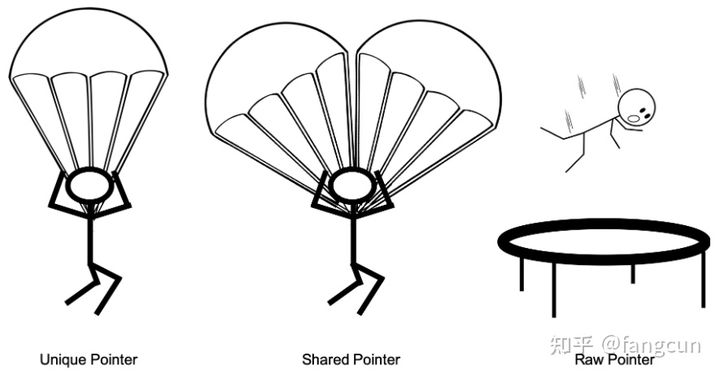
\includegraphics[scale=0.5]{img/1-3.jpg}
\end{figure}

\subsubsection*{建议}

\begin{itemize}
	\item 总是使用智能指针,不要直接使用原生指针。
	\item 对于单一所有权的对象使用unique\_ptr智能指针,对于需要共享所有权的对象使用shared\_ptr智能指针。对于可能出现的循环引用,使用weak\_ptr智能指针。
	\item 总是使用make\_unique()/make\_shared()来生成智能指针对象(也就是在对象创建后,立即生成智能指针引用它)。
	\item 不要继续使用已经废弃的auto\_ptr智能指针,使用unique\_ptr智能指针替换它。
	\item 如果要使用this指针生成shared\_ptr智能指针,应该考虑使用shared\_from\_this()。此外,不应该使用this指针生成unique\_ptr智能指针。
\end{itemize}

\subsection{哈希表和集合}

无序容器,比如哈希表可以提供O(1)时间复杂度的插入,查询和删除操作。我们可以将一个对象的属性进行组合,将其转换为一个整数类型的关键字,然后使用这一关键字作为键值访问哈希表。C++98为我们提供了map和set这两种哈希表的变种,它们可以提供O(lgN)时间复杂度的插入,查询和删除操作(标准库使用平衡二叉树来实现它们,所以时间复杂度不是哈希表的O(1))。map和set的优点是,它们中所存放的元素的排列是有序的,元素在容器中的位置由元素间进行小于比较运算得到。如果元素在容器中的顺序对我们不重要,使用无序容器显然是更好的选择。

C++11为我们提供了unordered\_map和unordered\_set(还有unordered\_multimap和unordered\_multiset)等无序容器。我们只需要为容器中存放的对象实现良好的哈希函数,就可以得到不错的插入,查询和删除操作的性能提升。对于标准库提供的对象,很多已经实现了哈希函数,我们不需要自己实现它。下面的代码使用unordered\_map实现了字符串到整数的映射:

\begin{lstlisting}[language={[ANSI]C},keywordstyle=\color{blue!70},commentstyle=\color{red!50!green!50!blue!50},frame=shadowbox, rulesepcolor=\color{red!20!green!20!blue!20},basicstyle=\small,numbers=left, numberstyle=\tiny,breaklines=true]
std::unordered_map<std::string, int> userToIndexMap;
\end{lstlisting}

\subsubsection*{建议}

\begin{itemize}
	\item 总是优先使用std::unordered\_map和std::unordered\_set作为无序容器,除非其它无序容器可以提供我们所需的额外功能,或是可以带来明显的性能提升。
	\item 优先使用std::unordered\_map和std::unordered\_set作为查询表,除非容器中元素的顺序对我们有用。
	\item 在某些情况下,比如表中元素较少时,哈希表的操作效率可能不如二叉树,甚至是顺序数组。
\end{itemize}

\newpage
\section{重要特性}

本章节介绍的特性对于我们来说非常重要。这些特性可以使我们的工作变得更加轻松,它们有的有利于我们捕获程序bug,有的让我们的代码变得更简洁,更容易阅读。

\subsection{代码安全性/错误捕获}

C++11为我们提供了一些新的语言特性使得我们在编译时就可以捕获一些代码逻辑上的错误。

\subsubsection{nullptr关键字}

对于使用C/C++的老程序员来说,NULL这个常量大家一定非常熟悉。毕竟,我们经常会遇到由它引发的段错误!NULL本质上是一个预定义的值为0的常量,并非C/C++语言的关键字,这就造成了一定问题。考虑下面的代码,printMe函数有两个版本。我们使用指针调用printMe函数,本应该调用printMe(const User* user)这一版本,但如果我们的参数是一个NULL指针,调用的实际上却是printMe(long int userIndex)这一版本。这是因为NULL的值实际上是0,0属于int类型,C/C++编译器认为printMe(long int userIndex)这一版本更加匹配。现在C++11为我们提供了nullptr这一关键字,可以完全避免这一问题。

\begin{lstlisting}[language={[ANSI]C},keywordstyle=\color{blue!70},commentstyle=\color{red!50!green!50!blue!50},frame=shadowbox, rulesepcolor=\color{red!20!green!20!blue!20},basicstyle=\small,numbers=left, numberstyle=\tiny,breaklines=true]
void printMe(long int userIndex); // prints user given index  
void printMe(const User* user); // prints user, or all if NULL  

printMe(NULL); // prints all users? NO
\end{lstlisting}

这样做:

\begin{lstlisting}[language={[ANSI]C},keywordstyle=\color{blue!70},commentstyle=\color{red!50!green!50!blue!50},frame=shadowbox, rulesepcolor=\color{red!20!green!20!blue!20},basicstyle=\small,numbers=left, numberstyle=\tiny,breaklines=true]
if (myPtr == nullptr || myOtherPtr == nullptr || myThirdPtr == nullptr) { // YES!!
	return nullptr; // YES!!  
}
\end{lstlisting}

不要这样做:

\begin{lstlisting}[language={[ANSI]C},keywordstyle=\color{blue!70},commentstyle=\color{red!50!green!50!blue!50},frame=shadowbox, rulesepcolor=\color{red!20!green!20!blue!20},basicstyle=\small,numbers=left, numberstyle=\tiny,breaklines=true]
if (myPtr == NULL || !myOtherPtr || myThirdPtr == 0) { // NO!!  
	return NULL; // NO!!
}
\end{lstlisting}

\subsubsection*{建议}

\begin{itemize}
	\item 不要设置指针变量的值为0或NULL。
	\item 使用新的nullptr关键字代替NULL。
\end{itemize}

\subsubsection{override关键字}

子类如果要覆盖父类的函数,我们需要将父类的函数定义为虚函数(virtual function),子类覆盖对应的虚函数,需要保证它和父类的虚函数完全匹配。很多时候,我们可能会因为疏忽而没有让两者完全匹配,造成难以察觉到bug,比如下面的代码:

\begin{lstlisting}[language={[ANSI]C},keywordstyle=\color{blue!70},commentstyle=\color{red!50!green!50!blue!50},frame=shadowbox, rulesepcolor=\color{red!20!green!20!blue!20},basicstyle=\small,numbers=left, numberstyle=\tiny,breaklines=true]
class User {
	virtual void print();  
	virtual string getName() const;  
	void performAction(const Action& a); // note: not virtual!
};
class PowerUser : User {
	void print(); // overrides User::print
	string getName(); // doesn't override User::getName - missing const
	void performAction(const Action& a); // doesn't override - base func not virtual  
};
\end{lstlisting}

C++11为我们提供了一个新的关键字override,可以避免这一问题。使用这一关键字的函数如果没有与之完全匹配的父类虚函数,编译器就会报告错误,我们就可以及时做出修改。下面的代码我们使用override关键字重写了PowerUser:

\begin{lstlisting}[language={[ANSI]C},keywordstyle=\color{blue!70},commentstyle=\color{red!50!green!50!blue!50},frame=shadowbox, rulesepcolor=\color{red!20!green!20!blue!20},basicstyle=\small,numbers=left, numberstyle=\tiny,breaklines=true]
class PowerUser : User {
	void print() override; // OK: overrides User::print
	string getName() override; // ERROR: wrong type
	void performAction(const Action& a) override; // ERROR: base func not virtual  
};
\end{lstlisting}

此外,C++11还为我们提供了final关键字,用于声明函数或类不可被覆盖或继承。使用这一关键字有助于编译器做出更好的优化。

\subsubsection*{建议}

\begin{itemize}
	\item 覆盖父类虚函数时,总是使用override关键字。
	\item 使用final关键字有助于编译器优化(虽然优化效果不明显)。
\end{itemize}

\subsubsection{控制类的默认行为}

编译器为了方便,会自动生成一些我们没有定义的函数。比如类的默认构造函数,复制构造函数,赋值运算函数,析构函数等等。对于复制构造函数来说,编译器生成的复制构造函数会遍历类的每个成员,然后执行对应的复制构造函数。一般来说,使用编译器自动生成的函数是个不错的选择,但有时候,我们的一些行为可能导致编译器不会为我们自动生成想要的函数,比如,如果我们自己定义了一个复制构造函数,编译器就不会再为我们自动生成移动构造函数,也就享受不到C++11带来的潜在的自动的性能提升。

显然,记忆编译器何时会自动生成这些函数,何时不会太过麻烦。所以,我们可以遵循这样的原则:如果有一个编译器可以自动生成的函数被我们自己定义的,那么所有其它可以自动生成的函数都应该进行显式标记。C++11允许我们使用default和delete关键字(default关键字标记的函数,编译器会自动生成,delete关键字标记的自动生成函数会被编译器移除)来对编译器可以自动生成的函数进行标记。

\begin{lstlisting}[language={[ANSI]C},keywordstyle=\color{blue!70},commentstyle=\color{red!50!green!50!blue!50},frame=shadowbox, rulesepcolor=\color{red!20!green!20!blue!20},basicstyle=\small,numbers=left, numberstyle=\tiny,breaklines=true]
class User {  
	User(const User&) = default; // accept default copy construction  
	User& operator= (const User&) = delete; // disallow copy assignment  
	User(User&&) = default; // accept default move constructor  
	User& operator= (User&&) = default; // accept default move assignment  
	~User() = default; // accept default destructor  
};
\end{lstlisting}

要么全部,要么一个都不,这一原则也适用于父类包含虚析构函数的情况。通常这种情况下,我们还应该使用delete关键字来移除复制构造函数,避免使用子类对象构造父类对象引发的数据损失。

\subsubsection*{建议}

我们可以使用下面的原则来避免错误发生:

\begin{itemize}
	\item 如果我们只需要编译器自动生成的函数(大多数情况下),要么不要对任一函数使用default标记,要么对所有函数使用default标记。
	\item 如果我们自己定义了任意一个编译器可以自动生成的函数(包括虚析构函数),对于其它自动生成函数,要么,我们自己定义它,要么使用default/delete对其进行标记。
	\item 使用delete标记子类不需要的父类函数,以及不需要的编译器自动生成的函数(之前C++98通过private关键字进行这一工作)。
\end{itemize}

\subsubsection{array数组}

C++11为我们带来了array数组,使用它不仅可以像普通的C风格数组一样利用栈空间。还可以利用标准库提供的一些模板算法:比如find(),count()等等。此外,因为array数组是一个类型,不会有像C风格数组一样有被编译器作为一个普通指针传给函数造成的潜在风险。考虑下面的代码,printMe函数的参数是一个指向User对象的指针,我们还定义了一个C风格的包含了50个User对象的数组,我们将数组作为参数可以调用printMe函数(C风格数组的数组名会被编译器认为是一个指针),调用结果是打印出了数组第一个元素的内容,显然,这和我们的本意不同,allUsers的字面意思是所有用户,我们更想要的是打印所有数组内元素的信息,但编译器没有提醒我们。

\begin{lstlisting}[language={[ANSI]C},keywordstyle=\color{blue!70},commentstyle=\color{red!50!green!50!blue!50},frame=shadowbox, rulesepcolor=\color{red!20!green!20!blue!20},basicstyle=\small,numbers=left, numberstyle=\tiny,breaklines=true]
printMe(User * user) { … }  // prints user pointer

User allUsers[50]; // native C-style array  
printMe(allUsers); // OOPS, only the first user is printed
\end{lstlisting}

使用array数组,我们可以在编译时就提前发现问题:

\begin{lstlisting}[language={[ANSI]C},keywordstyle=\color{blue!70},commentstyle=\color{red!50!green!50!blue!50},frame=shadowbox, rulesepcolor=\color{red!20!green!20!blue!20},basicstyle=\small,numbers=left, numberstyle=\tiny,breaklines=true]
array<User, 50> allUsers;  
printMe(allUsers); // ERROR - no matching function
\end{lstlisting}

\subsubsection*{建议}

\begin{itemize}
	\item 尽量使用std::array替代语言自带的固定大小的数组。
	\item 除非使用std::array会带来明显的性能下降。
	\item 通常,在开启常规的编译器优化后,std::array带来的性能下降非常小,甚至完全没有影响。
\end{itemize}

\subsubsection{\{\}初始化}

在之前,我们可以使用=运算符加上()构造函数,或\{\}来对变量进行初始化,但具体在何种情况使用何种方法初始化其实并不简单。C++11对\{\}初始化进行了扩展,让它可以用于任意情况的变量初始化。下面是使用\{\}进行变量初始化的三种形式:

\begin{lstlisting}[language={[ANSI]C},keywordstyle=\color{blue!70},commentstyle=\color{red!50!green!50!blue!50},frame=shadowbox, rulesepcolor=\color{red!20!green!20!blue!20},basicstyle=\small,numbers=left, numberstyle=\tiny,breaklines=true]
string username = {"Vader"};
string username{"Vader"};
string username = string{"Vader"};
\end{lstlisting}

目前,C++自带的容器都可以接收std::initializer\_list作为构造函数的参数,我们可以使用\{\}来对容器进行初始化,例子如下:

\begin{lstlisting}[language={[ANSI]C},keywordstyle=\color{blue!70},commentstyle=\color{red!50!green!50!blue!50},frame=shadowbox, rulesepcolor=\color{red!20!green!20!blue!20},basicstyle=\small,numbers=left, numberstyle=\tiny,breaklines=true]
vector<int> actionIndexes = {1, 2, 3, 4};
map<string, int> nameToIndexMap = { {"Vader", 1}, {"Skywalker", 1} };
\end{lstlisting}

需要注意的是,初始化列表构造函数会被优先匹配,读者可以考虑下面的代码,第一行代码调用的是普通的构造函数,生成了一个大小为5的vector对象,第二行代码调用的是初始化列表构造函数,生成了一个大小为1,第一个元素为5的vector对象。

\begin{lstlisting}[language={[ANSI]C},keywordstyle=\color{blue!70},commentstyle=\color{red!50!green!50!blue!50},frame=shadowbox, rulesepcolor=\color{red!20!green!20!blue!20},basicstyle=\small,numbers=left, numberstyle=\tiny,breaklines=true]
vector<int> v(5); // vector of size 5  
vector<int> v{5}; // vector with 1 value which is 5
\end{lstlisting}

我们可以在类定义中使用\{\}对成员变量进行初始化,使用这一方法可以避免在有多个构造函数时,忘记初始化某个成员变量。如果某一成员变量在构造函数也进行了初始化,构造函数中的初始化会代替类定义中的初始化。

\begin{lstlisting}[language={[ANSI]C},keywordstyle=\color{blue!70},commentstyle=\color{red!50!green!50!blue!50},frame=shadowbox, rulesepcolor=\color{red!20!green!20!blue!20},basicstyle=\small,numbers=left, numberstyle=\tiny,breaklines=true]
class User {  
	User() {} // don't need to initialize default here, already done  
	String username {"John Doe"};  
};
\end{lstlisting}

\subsubsection*{建议}

\begin{itemize}
	\item 使用{}来初始化容器,以及支持初始化列表的类对象。
	\item 为了避免和构造函数混淆,结合=运算符使用\{\}进行初始化。
	\item 对于其它变量使用构造函数或=运算符进行初始化。
	\item 在类成员变量定义的地方,使用\{\}对它进行初始化。
\end{itemize}

\subsection{更强大的功能}

一般来说,如果某个功能能够为绝大多数开发者带来好处,我们就会在未来将其加入C++标准。如果读者之前的某个功能是自己或着通过第三方库实现的,后来C++标准直接包含了这个功能,那么我们推荐读者使用C++标准提供的功能替换原来的实现。

\subsubsection{constexpr关键字}

现代C++倾向于在编译期就尽可能多地完成代码计算,直接将计算结果写入最终的二进制代码。这样做之后,程序运行时所需要实时计算的代码就会少很多,程序在性能表现上会提高不少。C++11引入了constexpr关键字,我们可以使用这一关键字来标记能够在编译期预计算的表达式。如果一个表达式被使用constexpr进行标记,它的计算不应该依赖于程序运行时才能确定的其它变量。但如果使用constexpr关键字对函数进行标记,函数参数允许使用运行时才能确定的变量,编译器会根据推断选择在编译时计算出结果,还是在运行时进行计算。比如下面的代码,使用常量4调用factorial函数,计算结果会在编译时预计算,使用变量someNumber调用factorial函数,计算在运行时进行。

\begin{lstlisting}[language={[ANSI]C},keywordstyle=\color{blue!70},commentstyle=\color{red!50!green!50!blue!50},frame=shadowbox, rulesepcolor=\color{red!20!green!20!blue!20},basicstyle=\small,numbers=left, numberstyle=\tiny,breaklines=true]
constexpr long long factorial(int n) {  
	return n <= 1 ? 1 : (n * factorial (n – 1));  
}
factorial(4); // 24 - computed at compile time!
factorial(someNumber); // slower, computed at run time!  
\end{lstlisting}

\subsubsection*{建议}

\begin{itemize}
	\item 对于静态的(static),并且不需要修改的类成员变量使用constexpr进行标记,而不是const。尽管对于整数类型的变量,两者的意义一样,但对于其它类型,使用constexpr更为准确。
	\item 尽量使用static constexpr标记的成员变量来替代\#define定义的宏,这样做既可以得到内联代码的好处,又保证了类型安全。
	\item 如果一个功能的结果可以在编译期预计算,考虑使用constexpr来优化性能表现。
\end{itemize}

\subsubsection{Lambda表达式}

很多时候,我们可能需要将自定义的函数传递给其它函数。为了简化这一过程,C++11为我们提供了Lambda表达式,可以在原地生成一个函数对象,它的基本形式如下:

\begin{lstlisting}[language={[ANSI]C},keywordstyle=\color{blue!70},commentstyle=\color{red!50!green!50!blue!50},frame=shadowbox, rulesepcolor=\color{red!20!green!20!blue!20},basicstyle=\small,numbers=left, numberstyle=\tiny,breaklines=true]
[capture list] (parameter list) { function body }
\end{lstlisting}

Lambda表达式的计算结果是一个std::function对象。下面的代码,演示了以往传递自定义函数的方法和使用Lambda表达式的方法。可以看出以往方法,是传递一个函数指针,自定义函数的代码和函数调用的地方距离较远,且自定义函数会暴露给其它无关部分。而现在的方法可以在调用函数的地方直接定义函数代码,不需要将自定义的函数暴露给其它无关部分。

\begin{lstlisting}[language={[ANSI]C},keywordstyle=\color{blue!70},commentstyle=\color{red!50!green!50!blue!50},frame=shadowbox, rulesepcolor=\color{red!20!green!20!blue!20},basicstyle=\small,numbers=left, numberstyle=\tiny,breaklines=true]
// Using named function
bool isLannister(const string& username) {  
	return username.find("Lannister") != string::npos;  
}  
int numLannisters = std::count_if(usernames.begin(), usernames.end(), isLannister);  

// Using lambda
int numLannisters = std::count_if(usernames.begin(), usernames.end(),  
[] (const string& username) {   
	return username.find("Lannister") != string::npos;  
});
\end{lstlisting}

之前,如果函数计算需要额外的变量,我们需要使用functor对象(一个重载()运算符的类对象)。现在有了Lambda表达式,我们可以非常简单地创建一个匿名的functor类对象(也叫做闭包,closure)。只需要将需要的变量以逗号进行分割,带上=(表示按值传递)或\&前缀(表示按引用传递)放置到Lambda表达式的中括号([])中即可。使用这一方法可以捕获所有局部变量,但不能捕获类成员变量(但可以通过捕获this指针来间接捕获)。另外,读者需要注意使用捕获可能会带来降低代码可读性,以及引用悬挂(Lambda表达式生成的functor对象调用()运算符时,引用对象已经不存在)的风险。

\begin{lstlisting}[language={[ANSI]C},keywordstyle=\color{blue!70},commentstyle=\color{red!50!green!50!blue!50},frame=shadowbox, rulesepcolor=\color{red!20!green!20!blue!20},basicstyle=\small,numbers=left, numberstyle=\tiny,breaklines=true]
struct Contains {  
	const string& substr;  
	Contains(const string& substr) : substr(substr) {}  
	bool operator () (const string& username) {  
		return username.find(substr) != string::npos; }  
};  
string stark = "Stark";  
int numStarks = std::count_if(usernames.begin(), usernames.end(), Contains(stark));  

int numStarks = std::count_if(usernames.begin(), usernames.end(), [&stark] (const string& username) {  
	return username.find(stark) != string::npos;  
});
\end{lstlisting}

一般来说,如果同一个函数被多次作为函数参数使用,或者它的代码行数较多,就不应该使用Lambda表达式来定义它。

\subsubsection*{建议}

\begin{itemize}
	\item 在大多数情况下,使用Lambda表达式可能会造成代码可读性下降。
	\item 在下面这些情况考虑使用Lambda表达式:
	\subitem 自定义函数需要访问局部变量。使用Lambda表达式要比使用functor对象或std::bind()更具可读性。
	\subitem 自定义函数的函数体非常简单(比如只有1-2行代码)。
	\subitem 自定义函数不会被多次使用。
	\item 使用Lambda表达式时:
	\subitem 不要使用捕捉所有模式(capture-all modes),而是在捕捉列表指定需要的变量。
	\subitem 为了可读性,建议不要在同一行定义Lambda表达式,而是将Lambda表达式定义在一个缩进后的新行,并对表达式的函数体缩进一级。
\end{itemize}

\subsubsection{原地构造插入}

对于很多标准库中的容器,比如vector,使用push\_back()插入一个新元素可能会调用不止一次构造函数。比如下面的代码,字符串字面量首先被作为参数构造了一个局部的string对象,然后,vector使用复制构造(copy-construct)函数生成了一个新的string对象,并将其放入了容器尾部。更好的选择是使用emplace\_back()函数,它会直接在vector容器的尾部生成对象,而不是先生成一个临时对象,然后将其复制到容器,最后清理掉临时对象。注意,为了获得性能提升,使用emplace应该使用被包含对象的构造函数的参数作为参数,而不是直接使用被包含对象的一个实例作为参数。考虑下面的代码:

\begin{lstlisting}[language={[ANSI]C},keywordstyle=\color{blue!70},commentstyle=\color{red!50!green!50!blue!50},frame=shadowbox, rulesepcolor=\color{red!20!green!20!blue!20},basicstyle=\small,numbers=left, numberstyle=\tiny,breaklines=true]
vector<string> users;  

// first makes string out of "Draco", then copy constructs into vector. Slower  
users.push_back("Draco");  

// direct construction in place. Faster  
users.emplace_back("Draco");   

// not faster since constructor explicitly called.  
users.emplace_back(string("Draco"));
\end{lstlisting}

\subsubsection*{建议}

下面这些情况,使用emplace替换掉push/insert可以获得性能表现提升:

\begin{itemize}
	\item 我们给插入函数传递的参数的类型和容器中存放的元素的类型不同。
	\item 容器允许插入的元素和已有元素重复,或着我们能够保证绝大多数情况下插入的元素和容器已有元素不同。
	\item 插入操作需要构造新对象。通常,除了在vector,deque或string的中间插入对象外,都满足这一情况。
\end{itemize}

\subsubsection*{并发}

C++11引入的一个重要特性就是对并发操作(Concurrency)的支持。之前因为C++标准并没有直接支持并发操作,人们使用boost或者POSIX这类第三方库完成并发操作。现在我们可以使用C++自带的并发库来完成相关操作。

\subsubsection{线程}

C++11为我们提供了非常简单的方法来创建线程(thread),只需要定义一个std::thread变量即可。在程序运行时,构造完这个变量,线程就自动开始并发执行。线程执行后,我们可以使用join()来等待它结束执行,也可以使用detach()来将其和创建它的线程分离。另外,我们还可以使用chrono库来对线程进行调度,在特定的时间唤醒线程。但需要注意的是,标准库并没有提供访问操作系统原始线程信息的API,比如线程的优先级等等。下面的代码演示了如何使用C++11来创建一个线程,线程在变量构造后会立刻执行。

\begin{lstlisting}[language={[ANSI]C},keywordstyle=\color{blue!70},commentstyle=\color{red!50!green!50!blue!50},frame=shadowbox, rulesepcolor=\color{red!20!green!20!blue!20},basicstyle=\small,numbers=left, numberstyle=\tiny,breaklines=true]
// spawn new thread that calls computeStuff()
std::thread workThread (computeStuff);
workThread.join(); // pauses until workThread completes
\end{lstlisting}

C++11还提供了thread\_local关键字允许我们将变量标记为线程局部变量。顾名思义,线程局部变量私有于单个线程,不同线程访问同一个线程局部变量,实际上访问的是不同的变量。相同线程访问同一个线程局部变量,访问结果是该线程上次对这一变量的操作结果。可以认为,每个线程都有独立的一份线程局部变量。

\subsubsection{原子变量}

多线程并发访问共享数据需要保证线程安全。而实现线程安全的最简单方法就是使用atomic库。C++自带的整数类型和指针类型都可以通过atomic库实现原子操作,其它类型只要满足trivially copyable定义,可以通过atomic模板实现来定义它的原子版本。下面的代码使用atomic模板定义了一个原子变量,我们对这一变量进行的后缀自增操作保证在多个线程间是原子的。

\begin{lstlisting}[language={[ANSI]C},keywordstyle=\color{blue!70},commentstyle=\color{red!50!green!50!blue!50},frame=shadowbox, rulesepcolor=\color{red!20!green!20!blue!20},basicstyle=\small,numbers=left, numberstyle=\tiny,breaklines=true]
std::atomic<int> latestUserId;  
int User::getGlobalUserId() {  
	return latestUserId++;  
}
\end{lstlisting}

\subsubsection{互斥锁}

除了原子变量,对于较长的代码,还可以使用mutex(互斥锁)来保证并发执行的正确性。当一个线程开始进入临界区,我们可以使用mutex加锁,等线程离开临界区,我们解锁,保证临界区的代码不会同时被多个线程执行。为了更加可靠,我们还可以结合使用unique\_lock和mutex,unique\_lock通过unique\_ptr来保证在析构时解锁mutex,从而避免只使用mutex的情况下,临界区代码抛出异常,mutex没有解锁而导致的死锁问题。需要注意的是mutex的操作代价较大,读者应该尽可能使用原子变量,只有在操作比较复杂时使用mutex。

\begin{lstlisting}[language={[ANSI]C},keywordstyle=\color{blue!70},commentstyle=\color{red!50!green!50!blue!50},frame=shadowbox, rulesepcolor=\color{red!20!green!20!blue!20},basicstyle=\small,numbers=left, numberstyle=\tiny,breaklines=true]
int latestUserId;  
std::mutex latestUserIdMutex;  
int User::getGlobalUserId() {  
	std::unique_lock<std::mutex> mutexLock(latestUserIdMutex);  
	return latestUserId++;  
} // mutex is released automatically here
\end{lstlisting}

\subsubsection{条件变量}

通过条件变量,我们可以将一个线程阻塞,直到另外一个线程将条件满足。因为条件变量需要被多个线程访问,我们需要结合mutex或其它并发访问保护措施来使用它。

\subsubsection{async}

C++11为我们引入了async(),使用它我们可以异步调用一个任务,并在未来需要的时候等待结果返回,相比于使用thread进行并发操作,它更方便,能够更好地利用CPU资源。需要注意的是,在默认调度策略下,调度器可以延迟任务执行,直到我们主动获取任务结果时才执行任务。我们可以将调度策略设置为launch::async来避免这一问题。

\subsubsection{future/promise}

调用async()会返回一个future对象。我们可以通过这一对象获取异步执行的任务的执行结果。因为任务是异步执行的,在获取结果时,任务未必已经执行完毕,所以我们调用future.get()后,调用线程就可能会阻塞等待任务执行完毕。当然,我们也可以选择执行其它任务,然后周期性检测任务是否已经执行完毕。另外,我们也可以在两个线程间使用类似的方式进行同步,只需要在一个线程创建一个promise对象,然后使用这一promise对象生成一个future对象,最后将生成的future对象传递给另一个线程,在另一个线程里我们就可以等待promise对象所代表的任务执行完毕。

\begin{lstlisting}[language={[ANSI]C},keywordstyle=\color{blue!70},commentstyle=\color{red!50!green!50!blue!50},frame=shadowbox, rulesepcolor=\color{red!20!green!20!blue!20},basicstyle=\small,numbers=left, numberstyle=\tiny,breaklines=true]
std::future<int> idFuture = std::async(getGlobalUserId);  
int userid = idFuture.get(); // waits for getGlobalUserId to return
\end{lstlisting}

\subsubsection*{建议}

并发编程是一个强大的工具,但用起来却非常容易出错。

\begin{itemize}
	\item 在考虑使用thread前,尝试使用async()和future对象。
	\item 为了线程安全,我们可以使用原子变量(场景非常简单的情况下)和mutex(处理复杂操作)。
	\item 使用future对象和promise对象可以很好地控制线程的执行,进行线程间的数据同步。
\end{itemize}

\subsubsection{正则表达式}

C++11引入了正则表达式。下面的代码演示了使用正则表达式将文本中的does not替换为does:

\begin{lstlisting}[language={[ANSI]C},keywordstyle=\color{blue!70},commentstyle=\color{red!50!green!50!blue!50},frame=shadowbox, rulesepcolor=\color{red!20!green!20!blue!20},basicstyle=\small,numbers=left, numberstyle=\tiny,breaklines=true]
string str("one does not simply use a regex");  
regex expr("does not");
str = std::regex_replace(str, expr, "does");
// "one does simply use a regex"
\end{lstlisting}

\subsubsection*{建议}

\begin{itemize}
	\item 考虑使用C++11引入的regex库进行正则表达式匹配。
	\item 较为的复杂的正则表达式可以通过原始字符串字面量(raw string literals)进行简化。
\end{itemize}

\subsubsection{计时工具}

C++标准通过chrono库为我们提供了计时工具。但C++11标准的chrono库,还不支持时区,UTC时间,TAI时间以及日历功能。所以,对于需要依赖日历的物理模拟应用,应该使用其它计时工具。

\subsubsection*{建议}

\begin{itemize}
	\item 使用C++的chrono库来代替原来的C计时库进行计时。
	\item 对于依赖日历的物理模拟应用,应该使用其它计时工具。
\end{itemize}

\subsubsection{随机分布生成器}

在游戏、自动化测试和模拟程序中我们经常需要用到伪随机数。以往,我们可能会使用C的rand()函数来生成一个随机数,然后对其进行模运算,从而获得0到某个整数范围的随机数。比如,使用下面的代码可以获得一个0到100范围内的伪随机数:

\begin{lstlisting}[language={[ANSI]C},keywordstyle=\color{blue!70},commentstyle=\color{red!50!green!50!blue!50},frame=shadowbox, rulesepcolor=\color{red!20!green!20!blue!20},basicstyle=\small,numbers=left, numberstyle=\tiny,breaklines=true]
int randInt = rand() % 101; // C-style
\end{lstlisting}

但是,通过这种方法生成的伪随机数并不是在0到100之间均匀分布的。对于需要自然随机分布的应用,比如进行蒙特卡洛模拟,使用这样的伪随机数会得到错误的结果。C++标准现在提供了一个更通用的随机分布生成器,只是使用它相较于使用rand()来说较为繁琐,如果随机数的分布不是很重要,读者可以继续使用rand()来生成随机数。下面是使用C++标准自带的随机分布生成器生成0到100的随机数:

\begin{lstlisting}[language={[ANSI]C},keywordstyle=\color{blue!70},commentstyle=\color{red!50!green!50!blue!50},frame=shadowbox, rulesepcolor=\color{red!20!green!20!blue!20},basicstyle=\small,numbers=left, numberstyle=\tiny,breaklines=true]
std::default_random_engine generator;  
std::uniform_int_distribution distribution(0, 100);  
int randInt = distribution(generator);
\end{lstlisting}

我们也可以通过std::bind()和auto来简化调用:

\begin{lstlisting}[language={[ANSI]C},keywordstyle=\color{blue!70},commentstyle=\color{red!50!green!50!blue!50},frame=shadowbox, rulesepcolor=\color{red!20!green!20!blue!20},basicstyle=\small,numbers=left, numberstyle=\tiny,breaklines=true]
auto randomGenerator = std::bind(distribution, generator);
int randInt = randomGenerator();
\end{lstlisting}

需要注意的是,C++标准自带的std::default\_random\_engine也有许多问题,如果读者对随机数的要求比较严格,建议使用PCG来生成伪随机数,它使用简单,只需要包含一个头文件,且生成随机数的效率更高。

\begin{itemize}
	\item 对于随机数的质量要求不高的应用,读者可以继续使用C库的rand()来生成伪随机数。
	\item 对于需要高质量合理分布的随机数的应用,读者应该使用C++标准带来的random库。
	\item 对于需要高质量随机数的应用,读者应该使用PCG来替换C++标准自带的std::default\_random\_engine。
\end{itemize}

\subsection{更好的编码体验}

C++11提供了一些非功能性的语法糖来帮助我们编码。

\subsubsection{auto关键字}

C++11提供了auto关键字来方便我们通过赋给变量的初始值的类型来确定变量的类型。

\begin{lstlisting}[language={[ANSI]C},keywordstyle=\color{blue!70},commentstyle=\color{red!50!green!50!blue!50},frame=shadowbox, rulesepcolor=\color{red!20!green!20!blue!20},basicstyle=\small,numbers=left, numberstyle=\tiny,breaklines=true]
auto hero = User("Geralt");  
User hero = User("Geralt");
\end{lstlisting}

类型自动推导对于类型名称特别长的情况特别适用:

\begin{lstlisting}[language={[ANSI]C},keywordstyle=\color{blue!70},commentstyle=\color{red!50!green!50!blue!50},frame=shadowbox, rulesepcolor=\color{red!20!green!20!blue!20},basicstyle=\small,numbers=left, numberstyle=\tiny,breaklines=true]
unordered_map<string, User>::const_iterator userIt = userLookupMap.find("Geralt");  
// VS.
auto userIt = userLookupMap.find("Geralt");
\end{lstlisting}

另一种比较常见的用法是在for循环中使用类型自动推导:

\begin{lstlisting}[language={[ANSI]C},keywordstyle=\color{blue!70},commentstyle=\color{red!50!green!50!blue!50},frame=shadowbox, rulesepcolor=\color{red!20!green!20!blue!20},basicstyle=\small,numbers=left, numberstyle=\tiny,breaklines=true]
// Confusing - is user a User, std::string, int userid??
for (const auto& user : users) { ... }
\end{lstlisting}

使用auto关键字定义变量有许多好处:减少需要键入的代码;强迫人们必须对变量进行初始化;方便以后重构代码;减少类型转换bug等等。另外,在编写部分模板代码、Lambda表达式代码时,如果没有auto关键字,写起来也要麻烦许多。

需要注意的是使用auto关键字会降低代码可读性。考虑变量类型大量被auto关键字代替,人们想要得知类型信息可能需要跳转多个源文件。此外,auto关键字也会降低IDE(集成开发环境)对变量类型的识别,从而造成IDE的智能提示失效。

\subsubsection*{建议}

在下面这些情况可以使用auto关键字让编译器自动推导变量类型:

\begin{itemize}
	\item 变量类型非常复杂,本身可读性就低。
	\item 没有合适的类型别名来描述复杂的变量类型。
	\item 变量的类型对于读代码的人来说非常明显的情况。
\end{itemize}

\subsubsection{枚举类(Enum Class)}

C++11为我们提供了枚举类(Enum Class)。相较于枚举类型,它的成员不会被隐式转换为整数类型,可以保证类型安全。当我们需要成员的整数值时,也可以使用static\_cast()来进行类型转换。此外,我们需要通过类似FruitType::APPLE的形式来访问它的成员,要比枚举类型可以直接以类似FRUIT\_TYPE\_APPLE的形式访问要更好,更不容易出现命名冲突。我们还可以在枚举类的名称后指定成员的类型,默认情况下,枚举类的成员的值为int类型。最后,需要注意的是,枚举类不是一个正常意义的类,它不能包含有函数,也不能继承和被继承。

\begin{lstlisting}[language={[ANSI]C},keywordstyle=\color{blue!70},commentstyle=\color{red!50!green!50!blue!50},frame=shadowbox, rulesepcolor=\color{red!20!green!20!blue!20},basicstyle=\small,numbers=left, numberstyle=\tiny,breaklines=true]
enum class FruitType : char {APPLE, ORANGE, PEAR};
int numUsers = FruitType::APPLE; // Doesn't compile – correctly!
\end{lstlisting}

\subsubsection*{建议}

\begin{itemize}
	\item 我们可以使用枚举类(Enum Class)来保证类型安全,减少命名冲突。
	\item 我们应该在定义枚举类时给出它的成员的类型,这样做既避免了可能的误用,又减少了内存使用。
\end{itemize}

\subsubsection{基于范围的for循环}

C++11为我们提供了一个新的for循环语法用于遍历容器。相比于之前遍历容器的方法,使用它更为高效。但需要注意的是,如果我们需要对遍历的容器进行修改,或是需要正在遍历的元素的索引,可能基于范围的for循环就不太适用了。下面的代码给出了使用它的示例:

\begin{lstlisting}[language={[ANSI]C},keywordstyle=\color{blue!70},commentstyle=\color{red!50!green!50!blue!50},frame=shadowbox, rulesepcolor=\color{red!20!green!20!blue!20},basicstyle=\small,numbers=left, numberstyle=\tiny,breaklines=true]
// Off-by-one-bug prone
for (int k=0; k<allUsers.size(); k++) {
	doSomething(allUsers[k]);
}  

// Blech, too long
for(vector<User>::const_iterator it=allUsers.begin(); it!=allUsers.end(); it++){
	doSomething(it);
}
// Too complicated
std::for_each(allUsers.begin(), allUsers.end(), doSomething);

// Nice and clean!
//  Also reminds reader of the container elements' type
for (const User& user : allUsers) {
	doSomething(user);
}
\end{lstlisting}

虽然我们可以在基于范围的for循环中使用auto关键字来进行类型自动推导,但这样做可能会给阅读代码的人带来困惑,所以不推荐这样:

\begin{lstlisting}[language={[ANSI]C},keywordstyle=\color{blue!70},commentstyle=\color{red!50!green!50!blue!50},frame=shadowbox, rulesepcolor=\color{red!20!green!20!blue!20},basicstyle=\small,numbers=left, numberstyle=\tiny,breaklines=true]
// Confusing - is user a User, std::string, integer userid??
for (const auto& user : allUsers) { ... }
\end{lstlisting}

使用基于范围的for循环,我们需要注意下面这些细节:

\begin{itemize}
	\item 对于不需要修改的类对象,使用const \&来接收元素。
	\item 对于需要修改的容器元素,使用\&来接收元素。
	\item 对于元素类型是基本变量类型的,且不需要修改的情况,使用值传递来接收元素。
\end{itemize}

下面的代码给出了基于范围的for循环的一些例子:

\begin{lstlisting}[language={[ANSI]C},keywordstyle=\color{blue!70},commentstyle=\color{red!50!green!50!blue!50},frame=shadowbox, rulesepcolor=\color{red!20!green!20!blue!20},basicstyle=\small,numbers=left, numberstyle=\tiny,breaklines=true]
// 1. Read-only class object
for(const User& user: allUsers) {}

// 2. Modifiable class object
for(User& userToEdit: allUsers) {}

// 3. Read-only primitive
for(int userid: userids) {}
\end{lstlisting}

\subsubsection*{建议}

\begin{itemize}
	\item 考虑使用基于范围的for循环来遍历容器
	\item 除非一些特殊原因:
	\subitem 需要对容器进行修改
	\subitem 需要元素索引
	\subitem 需要双向遍历
	\item 为接收变量选用合适的限定符
	\item 不要使用auto关键字来自动推导元素类型
\end{itemize}

\subsubsection{类型别名}

以往,我们使用typedef关键字来给名称比较繁琐的类型起别名。但这种方法不支持模板,当起别名的是一个函数指针类型时也容易造成歧义。现在,我们可以使用using关键字来做这件事,它可以避免上述问题。下面的代码给出了使用这一关键字的示例:

\begin{lstlisting}[language={[ANSI]C},keywordstyle=\color{blue!70},commentstyle=\color{red!50!green!50!blue!50},frame=shadowbox, rulesepcolor=\color{red!20!green!20!blue!20},basicstyle=\small,numbers=left, numberstyle=\tiny,breaklines=true]
// template "typedef" allowed in C++11  
template <class T>  
using StringMap = std::map<std::string, T>; // Only in C++11  

// valid C++98 - confusing  
typedef bool (*compare)(int, int);

// valid C++11 - less confusing  
using compare = bool (*)(int, int);
\end{lstlisting}

\subsubsection*{建议}

\begin{itemize}
	\item 使用using替代typedef来定义类型别名。
\end{itemize}

\subsubsection{委托构造函数}

我们可以在定义构造函数时指定调用其它构造函数:

\begin{lstlisting}[language={[ANSI]C},keywordstyle=\color{blue!70},commentstyle=\color{red!50!green!50!blue!50},frame=shadowbox, rulesepcolor=\color{red!20!green!20!blue!20},basicstyle=\small,numbers=left, numberstyle=\tiny,breaklines=true]
class User {
	User(string name) {…} // name passed in
	User() : User("Jane Doe") {} // constructor delegation
};
\end{lstlisting}

\subsubsection*{建议}

\begin{itemize}
	\item 使用委托构造函数来减少不必要的代码重复。
\end{itemize}

\subsubsection{继承构造函数}

类似于委托构造函数,在子类没有额外增加成员变量的情况下,我们也可以使用using关键字直接指定父类的所有构造函数作为子类构造函数。示例如下:

\begin{lstlisting}[language={[ANSI]C},keywordstyle=\color{blue!70},commentstyle=\color{red!50!green!50!blue!50},frame=shadowbox, rulesepcolor=\color{red!20!green!20!blue!20},basicstyle=\small,numbers=left, numberstyle=\tiny,breaklines=true]
class PowerUser : public User {  
	using User::User; // PowerUser inherits User constructors  
	// VS
	PowerUser() : User() {} // call User constructor manually
};
\end{lstlisting}

\subsubsection*{建议}

\begin{itemize}
	\item 在子类没有额外增加成员变量的情况下,使用using关键字直接指定父类的所有构造函数作为子类构造函数,让代码更简洁。
	\item 其它情况下,应该在定义子类的构造函数时显式调用需要的父类构造函数。
\end{itemize}

\newpage
\section{次要特性}

本章节主要介绍一些不太重要,但需要我们了解的新特性。

\subsection{std::algorithm的增强}

C++11自带的algorithm库对[all|any|none]\_of,is\_sorted(),以及min/max做了增强,现在它们都可以接收任意长度的初始化列表作为参数。

\subsubsection*{建议}

\begin{itemize}
	\item 了解algorithm库的增强功能。
\end{itemize}

\subsection{单链表(Forward List)}

C++11提供了一个新的容器forward\_list。它的实现是一个单链表,适合用于单向遍历的场景。此外,它并不记录容器中的成员个数,对容器中的元素个数进行计数需要遍历整个链表,速度较慢。

\subsubsection*{建议}

\begin{itemize}
	\item 如果不能确定所需容器空间大小,以及希望任意的插入操作都不会影响外部引用的有效性,使用list。
	\item 其它情况,vector通常是最佳选择。
	\item 如果不需要反向遍历、经常查询容器中元素个数,也不需要进行任意的删除操作,考虑使用forward\_list来提高性能表现。
\end{itemize}

\subsection{元组(Tuple)}

一个元组(tuple)是一个紧凑存放N个值的序列,也可以认为元组(tuple)就是一个未命名的结构体。C++为我们提供make\_tuple()来生成元组(tuple)。由于元组(tuple)可以存放任意数据,且元组(tuple)这个名字不具有例如vector,list这类名字能够提示数据存储和逻辑结构的意义,我们应该谨慎使用它,避免引起他人阅读代码时的困惑。

\subsubsection*{建议}

除了下列情况,尽量使用带有名称的类/结构体:

\begin{itemize}
	\item 除了进行编译,类型名称很难确定的情况(比如进行模板编程)。
	\item 没有有意义的名称可以命名。
	\item 数据的生命周期很短,只有很少很局部的代码用到,命名它们对可读性也不会有所提高。
\end{itemize}

\subsection{>>符号}

对于C++98来说,>>符号表示向右位移运算,如果>>符号中间有空格,则代表模板类型匹配结束。参考下面代码:

\begin{lstlisting}[language={[ANSI]C},keywordstyle=\color{blue!70},commentstyle=\color{red!50!green!50!blue!50},frame=shadowbox, rulesepcolor=\color{red!20!green!20!blue!20},basicstyle=\small,numbers=left, numberstyle=\tiny,breaklines=true]
set<pair<int, int> > pairSet; // C++98 and C++11  
set<pair<int, int>> pairSet; // C++11 ONLY
\end{lstlisting}

\subsubsection*{显式转换}

对于C++98来说,我们可以对构造函数使用explicit关键字来禁止使用该构造函数进行隐式转换。C++11对转换运算做了扩展,比如,如果想要在if语句中使用其作为判断条件,可以这样做:

\begin{lstlisting}[language={[ANSI]C},keywordstyle=\color{blue!70},commentstyle=\color{red!50!green!50!blue!50},frame=shadowbox, rulesepcolor=\color{red!20!green!20!blue!20},basicstyle=\small,numbers=left, numberstyle=\tiny,breaklines=true]
class User
{
	operator bool()
	{
		return this->isValid();
	}
};

// Now User objects can be used like this
if (user)
{
	...
}

// ... But also like this??
int someNum = user;
\end{lstlisting}

但如上面代码,user也可以赋给int类型的someNum,这很可能引发bug。我们可以在bool函数前加上explicit关键字来禁止隐式转换:

\begin{lstlisting}[language={[ANSI]C},keywordstyle=\color{blue!70},commentstyle=\color{red!50!green!50!blue!50},frame=shadowbox, rulesepcolor=\color{red!20!green!20!blue!20},basicstyle=\small,numbers=left, numberstyle=\tiny,breaklines=true]
class User
{
	explicit operator bool()
	{
		return this->isValid();
	}
};

// Compile error - cannot convert User to int!
int someNum = user;
\end{lstlisting}

\subsubsection*{建议}

使用explicit关键字来避免隐式转换可能带来的问题。

\subsection{noexcept关键字}

通过使用noexcept关键字,我们可以将函数标记为不会抛出异常,从而方便编译器做出更好的优化。对于使用了noexcept关键字的函数,如果实际抛出了异常,会导致程序立即结束。

\subsubsection*{建议}

大多数情况下,可以忘掉noexcept关键字。但对于我们自定义的移动构造函数应该尽可能地使用它。此外,在有余力的情况下,可以考虑通过它来做性能优化。

\subsection{属性}

我们可以通过[[attribute]]的方式来给编译器提供一些提示信息,帮助编译器进行推断。对于C++11来说,它只有一个算是有用的[[noreturn]]属性来帮助编译器优化,但这一属性的作用也并不大。通常,我们只在很少的情况下使用[[noreturn]]来屏蔽编译器的错误警告。

\subsubsection*{建议}

对于C++11来说,不要使用它。

\newpage
\section{用于模板库开发的特性}

C++的许多高级特性主要用于模板库的开发。对于普通程序员来说,这些用于开发模板库的特性只需要了解即可。

\subsection{decltype()运算符}

C++11为我们提供了decltype()运算符来返回表达式的类型。比如 decltype(42ULL)返回的结果是unsigned long long。在之前,gcc编译器提供了一个类似的typeof运算符,现在我们完全可以使用decltype替换掉它。这一运算符通常用于模板函数,用于确定我们无法提前预知的模板函数的返回值的类型。对于不能确定类型的用于变量初始化的表达式,使用auto关键字是更好的选择。

\subsection{后缀返回类型语法(Suffix return type syntax)}

考虑下面代码中定义的add模板函数。我们应该怎样设置函数的返回类型?对于string和char*的加法运算结果是string类型,对于double和int的加法运算结果是double类型,对于QueryResult和QueryResult的加法运算结果可能是MultiQueryResult类型。

\begin{lstlisting}[language={[ANSI]C},keywordstyle=\color{blue!70},commentstyle=\color{red!50!green!50!blue!50},frame=shadowbox, rulesepcolor=\color{red!20!green!20!blue!20},basicstyle=\small,numbers=left, numberstyle=\tiny,breaklines=true]
template <typename Type1, typename Type2>  
??? add (Type1 x, Type2 y) {  
	return x + y;  
}
\end{lstlisting}

C++为我们提供了后缀返回类型语法来解决这一问题。我们可以直接通过后缀返回类型语法将返回值的类型设置为decltype()运算符的运算结果(使用后缀语法的原因是,编译器处理后缀语法时可以利用模板函数的参数x和参数y的信息,而前缀语法,编译器无法通过参数x和参数y来获取返回类型)。示例代码如下:

\begin{lstlisting}[language={[ANSI]C},keywordstyle=\color{blue!70},commentstyle=\color{red!50!green!50!blue!50},frame=shadowbox, rulesepcolor=\color{red!20!green!20!blue!20},basicstyle=\small,numbers=left, numberstyle=\tiny,breaklines=true]
template <typename Type1, typename Type2>  
auto add (Type1 x, Type2 y) -> decltype (x + y) {  
	return x + y;  
}
\end{lstlisting}

\subsection{可变参数模板}

C++11为我们引入了一个新的定义可变参数函数的方式,相较于printf函数使用的C风格可变参数函数定义,使用这种方式定义可变参数函数可以保证类型安全。示例如下:

\begin{lstlisting}[language={[ANSI]C},keywordstyle=\color{blue!70},commentstyle=\color{red!50!green!50!blue!50},frame=shadowbox, rulesepcolor=\color{red!20!green!20!blue!20},basicstyle=\small,numbers=left, numberstyle=\tiny,breaklines=true]
template <typename T>  
T adder(T v) { // base case  
	return v;  
}  
// Variadic template  
template <typename T, typename... Args>  
T adder(T first, Args... args) { // recursive case  
	return first + adder(args…); // 'peel off' more arguments  
}
\end{lstlisting}

可以看出,在上面的代码中,我们通过递归定义了一个可变参数的模板函数。读者不必担心递归定义会影响性能,它的递归计算是在编译期进行的,通常会比C风格定义更快。C++标准库中的tuple,make\_shared()和emplace\_back()能够得以实现,可变参数模板的支持功不可没。

\subsection{元编程:类型特征和静态断言}

元编程的用途主要是通过代码来让编译器自动生成更多的代码。对于C++来说,我们可以通过模板特化实现元编程,也就是在编译时由编译器自动生成新的类/函数。下面的代码通过元编程的方式实现了编译期计算阶乘:

\begin{lstlisting}[language={[ANSI]C},keywordstyle=\color{blue!70},commentstyle=\color{red!50!green!50!blue!50},frame=shadowbox, rulesepcolor=\color{red!20!green!20!blue!20},basicstyle=\small,numbers=left, numberstyle=\tiny,breaklines=true]
template <unsigned int n>  
struct factorial {  
	enum { value = n * factorial<n - 1>::value };
};  

template <>  
struct factorial<0> {  
	enum { value = 1 };
};  

unsigned int result=factorial<4>::value // 24 – computed at compile time!
\end{lstlisting}

C++为我们提供了多个type\_traits(类型特征)来方便我们在编译期获取类型特征,实现元编程。比如,我们可以通过is\_integral()判断一个类型是否是整型,通过is\_assignable()判断一个类型是否可以赋值给另一个类型,通过is\_pointer()判断一个类型是否是指针。当我们使用类型特征判断传递的类型不匹配我们的代码时,我们还可以通过static\_assert生成编译期错误。

\subsection{其它}

C++11允许局部和未命名的类型作为模板参数(之前不可以这样做)。另外,注意通过extern关键字来声明外部已经特化的模板代码,避免每个编译单元都生成一份相同的特化模板代码。

C++11的functional库为我们提供了function对象,用于表示可以被调用的对象(比如函数,函数指针,函数对象)。还为我们提供了bind()函数用于将特定变量和函数绑定生成一个新的function对象。

\subsubsection*{建议}

\begin{itemize}
	\item 阅读本文提供的参考资料,来更好地理解元编程。
	\item 如果模板函数的返回值的类型依赖于某个表达式,使用后缀返回类型语法和decltype()来定义模板函数的返回值类型。
	\item 对于一般的变量定义,使用auto关键字比decltype()更合适。
	\item 对于普通程序员来说,元编程的用处不大,对于硬核的通用库开发者,元编程是一个不错的工具。
\end{itemize}

\newpage
\section{不常用的高级特性}

本章节主要对C++11的一些比较高级,但很少使用的新特性进行简要介绍。

\subsection{引用包装(Reference Wrapper)}

我们可以通过std::reference\_wrapper来对引用进行包装,当对包装后的引用对象使用赋值运算,且运算参数是一个新的引用对象时,它会替换掉原来引用的对象,而不是执行引用对象本身的赋值运算。利用上面这一特性,我们可以在容器中存储引用包装对象,从而间接达到存储引用对象的目的。

\subsection{原始字符串字面量}

C++11为我们带来了正则表达式的支持,但正则表达式使用的$\backslash$符号,在C++的字符串字面量中具有转义的作用,需要两个$\backslash$符号才能转义为正则表达式的单个$\backslash$符号。显然,这样非常不便,所以C++11为我们提供了原始字符串字面量,我们只需要使用R"(...)"来包括字符串,字符串中的$\backslash$符号就不会被转义。

\begin{lstlisting}[language={[ANSI]C},keywordstyle=\color{blue!70},commentstyle=\color{red!50!green!50!blue!50},frame=shadowbox, rulesepcolor=\color{red!20!green!20!blue!20},basicstyle=\small,numbers=left, numberstyle=\tiny,breaklines=true]
比如R"(\w\\\w)"等价于C++字符串"\\w\\\\\\w"。
\end{lstlisting}

\subsection{用户定义字面量}

现在我们可以通过""运算符来定义类似浮点数12.F、16进制数0xab这样的字面量。通过这一特性我们可以将类似5km、5m的字符串变成对C++来说有意义的字面量。

\subsection{Unicode字符}

C++11引入了char16\_t(用于UTF-16)和char32\_t(用于UTF-32)两个类型来存储Unicode字符。我们可以使用u""(用于UTF-16)和U""(用于UTF-32)标记字符串按照Unicode编码进行存储。

\subsection{内联名字空间}

C++11允许使用inline关键字将名字空间标记为内联。内联名字空间中的成员自动成为其外部名字空间的成员。通常,我们使用这一特性来对代码进行版本控制(比如选择性的暴露不同版本的库代码作为默认实现)。

\subsection{带有生命周期的分配器}

现在自定义的分配器也可以包含有状态信息。我们可以通过这一特性实现一些特殊的分配策略。

\subsection{手动内存对齐}

C++11提供了alignas关键字来方便我们设置指定参数的内存对齐方式。

C++11提供了alignof关键字来方便我们获取指定参数内存对齐方式。

\subsection{quick\_exit}

调用quick\_exit()函数可以直接跳过析构函数的执行,立即结束程序运行。

此外,我们可以使用at\_quick\_exit()函数注册需要在quick\_exit()函数调用后执行的函数。

使用exit()则不会影响析构函数的执行。

使用abort()则以异常的方式中断程序运行。

\subsection{\_\_cplusplus}

\_\_cplusplus的值现在被设置为一个大于199711L的数字,对于符合C++11标准的编译器来说,这个值几乎可以认为是201103L。

\end{document}
